% ---------
%  Compile with "pdflatex hw1".
% --------
%!TEX TS-program = pdflatex
%!TEX encoding = UTF-8 Unicode

% Template borrowed from Jeff Erickson.

\documentclass[11pt]{article}
\usepackage[utf8]{inputenc}		% Allow some non-ASCII Unicode in source
\usepackage{jeffe, handout,graphicx}
\usepackage{forest}
\usepackage{mathtools}
\usepackage{cnn}
\usepackage{subfigure}
\usepackage{comment}


% =========================================================
%   Define common stuff for solution headers
% =========================================================
\Class{CS 6301.503}
\Semester{Spring 2019}
\Authors{1}
\AuthorOne{Scott C. Waggener}{scw180000}
%\Section{}

% =========================================================
\begin{document}
\HomeworkHeader{6 (Design)}{1}% homework number, problem number
% ---------------------------------------------------------
Read
\begin{solution}
	Complete
\end{solution}

% =========================================================
\HomeworkHeader{6 (Design)}{2}% homework number, problem number
% ---------------------------------------------------------
Read
\begin{solution}
	Complete
\end{solution}

% =========================================================
\HomeworkHeader{6 (Design)}{3}% homework number, problem number
% ---------------------------------------------------------
Read
\begin{solution}
	Complete
\end{solution}

% =========================================================
\HomeworkHeader{6 (Design)}{4}% homework number, problem number
% ---------------------------------------------------------
Read
\begin{solution}
	Complete
\end{solution}

% =========================================================
\HomeworkHeader{6 (Design)}{5}% homework number, problem number
% ---------------------------------------------------------
Compute the receptive field size at the input to the global average pooling layer for ResNet 50.

\begin{solution}
	$164\times164$
\end{solution}
\begin{proof}

	Looking at the architecture of Resnet-50 we see that there are a total of
	six downsamplings, each of which alter receptive field. Four of the
	downsamplings take place in the body, and two in the head. The body
	downsamplings are $3\times3/2$ and the head downsamplings are $3\times3/2$
	and $7\times7/2$. We can then compute receptive field by starting with $1$,
	multiplying by stride and adding filter size minus one.

	\begin{align}
		\text{conv5} &= 1 \\
		\text{conv4} &= \big(\text{conv5}+2\big)*2 = 6  \\
		\text{conv3} &= \big(\text{conv4}+2\big)*2 = 16  \\
		\text{conv2} &= \big(\text{conv3}+2\big)*2 = 36  \\
		\text{max pool} &= \big(\text{conv2}+2\big)*2 = 76  \\
		\text{conv1} &= \big(\text{max pool}+6\big)*2 = 164  \\
	\end{align}

	\noindent
	This result seems resonable, as it captures enough of the original image to
	resolve an object. It seems difficult to find solutions to sample
	calculations for full networks, \textbf{additional problems with verifiable
	solutions would be helpful}.

\end{proof}

% =========================================================
\HomeworkHeader{6 (Design)}{6}% homework number, problem number
% ---------------------------------------------------------
\begin{enumerate}[(a)]
	\item How does the accuracy of the half wide version copare to the original
		version?
	\begin{solution}
		The accuracy at the final epoch for the full and half versions are
		\begin{align}
			\text{Full} &= 91.03\%
			&
			\text{Half} &= 89.31\%
		\end{align}
	\end{solution}

	\item How long does an epoch of training take for both versions?
	\begin{solution}
		The times for epoch $3$ for both models (trained on GTX970) are
		\begin{align}
			\text{Full} &= 59s
			&
			\text{Half} &= 36s
		\end{align}
	\end{solution}

	\item Approximate how feature map memory, filter memory, and compute change
		between the full and half width versions.
	\begin{solution}

		\begin{align}
			&\text{Feature map memory} = \frac{1}{2}
			\\
			&\text{Filter memory} = \frac{1}{4}
			\\
			&\text{Compute} = \frac{1}{4}
		\end{align}
	\end{solution}
	\begin{proof}

		In our approximation we can look primarily at how convolutional layers will
		be affected, as such layers comprise the bulk of the network. In this case
		we know that

		\begin{align}
			\text{Filter Memory} &= N_o * N_i * F_r * F_c + N_o \\
			\text{Feature Map Memory} &= N_{o/i} * L_r * L_c\\
		\end{align}

		As such we expect to see a $1/2$ reduction in feature map memory, which
		makes sense given that the half wide version will store half as many
		feature maps. We also expect a $1/4$ reduction in filter coefficient
		memory as we are now mapping across $N_i=1/2$ and $N_o=1/2$ for a
		combined $1/4$ reduction.
		\newline

		For compute of 2D convolution we have

		\begin{align}
			\text{Compute Memory} &= N_o * N_i * L_r * L_c * F_r * F_c
		\end{align}

		which again contributes to a quarter reduction over $N_o * N_i$.


	\end{proof}

\end{enumerate}
% =========================================================
\HomeworkHeader{6 (Design)}{7}% homework number, problem number
% ---------------------------------------------------------
\begin{solution}
	The network design will be based on Inception v4. To inform our choice
	of network architecture we can use the given hint for an expected input
	global average pooling and think backwards from here. Obviously for
	CIFAR-10 we will have $10$ classes, so we need to choose $N_i$ to global
	average pooling somewhere above $10$, call it $30$. We will aim for $7
	\times 7$ spatial input to average pooling.
	\newline

	\noindent
	Again, recall that downsampling is given by
	\begin{align}
		M = \frac{L - F + 2P}{S}+1
	\end{align}

	\noindent
	Putting this together, our architecture looks like

\begin{figure}[H]
	\noindent\resizebox{\textwidth}{!}{
	\begin{tikzpicture}
		\def\groupsep{0.4cm}

		% Input
		\pic[inp] (input) at (0,0,0) {
				pic conv2d={res 3 depth 0.2}
		};
		\pic[inp] (input) at (0,0,0) {
				pic cnn/dims/above={res 3 depth 0.2 to 4
				text $3\times 32\times 32$
			}
		};
		\pic[inp] (input) at (0,0,0) {
				pic cnn/dims/below={res 3 depth 0.2 to -2
				text Input
			}
		};

		% Simple tail
		\pic[tail, right=\groupsep of input-south east] (tail)  {
			pic conv2d={res 3 depth 0.2}
		};
		\pic[tail, right=\groupsep of input-south east] {
				pic cnn/dims/above={res 3 depth 0.2 to 4
				text $64\times 32\times 32$
			}
		};
		\pic[tail, right=\groupsep of input-south east] {
				pic cnn/dims/below={res 3 depth 0.2 to -2
				text Tail $7\times7$
			}
		};

		% Inception A
		\pic[cnn, right=\groupsep+1*0.4cm of tail-south east] {
			pic cnn/dims/above={res 3 depth 0.2 to 4
				text $64\times 32\times 32$
			}
		};
		\pic[cnn,right=\groupsep of tail-south east,
			pic text=$4\times$ A] (A) {
			pic conv2d/repeat/decorate={res 3 depth 0.2 repeat 4 sep 0.2}
		};

		% Reduction A
		\pic[pool, right=\groupsep of A-south east] (A2)  {
			pic conv2d={res 2 depth 0.4}
		};
		\pic[pool, right=\groupsep of A-south east]  {
			pic cnn/dims/above={res 2 depth 0.4 to 4
				text $128 \times 15 \times 15$
			}
		};
		\pic[pool, right=\groupsep of A-south east]  {
			pic cnn/dims/below={res 2 depth 0.4 to -2
				text Reduction A \\ $3 \times 3 / 2$
			}
		};

		% Inception B
		\pic[cnn, pic text=$7\times$ B,
			right=\groupsep of A2-south east]
		(B) {
			pic conv2d/repeat/decorate={res 2 depth 0.4 repeat 7 sep 0.2}
		};
		\pic[cnn, right=\groupsep+3*0.6cm of A2-south east] {
			pic cnn/dims/above={res 2 depth 0.4 to 4
				text $128 \times 15 \times 15$
			}
		};

		% Reduction B
		\pic[pool, right=\groupsep of B-south east] (B2){
			pic conv2d={res 1 depth 0.6}
		};
		\pic[pool, right=\groupsep of B-south east]   {
				pic cnn/dims/above={res 1 depth 0.6 to 4
				text $256\times7\times7$
			}
		};
		\pic[pool, right=\groupsep of B-south east]   {
				pic cnn/dims/below={res 1 depth 0.6 to -2
				text Reduction B \\ $3 \times 3 / 2$
			}
		};

		% Inception C
		\pic[cnn, right=\groupsep+1*0.8cm of B2-south east] {
			pic cnn/dims/above={res 1 depth 0.6 to 4
				text $256\times7\times7$
			}
		};
		\pic[cnn, pic text=$3 \times$ C,
			right=\groupsep of B2-south east] (C)  {
			pic conv2d/repeat/decorate={res 1 depth 0.6 repeat 3 sep 0.2}
		};


		% Global avg
		\pic[vec, right=\groupsep of C-south east] (avg)  {
				pic vec={res 3 depth 0.25}
		};
		\pic[vec, right=\groupsep of C-south east]  {
				pic cnn/dims/front={res 3 depth 0.25 to 4
				text $256\times1\times1$
			}
		};
		\pic[vec, right=\groupsep of C-south east]  {
				pic cnn/dims/below={res 3 depth 0.25 to -2
				text Global Avg
			}
		};
		\def\groupsep{0.2cm}

		% Fully connected
		\pic[vec, right=\groupsep of avg-south east] (fc)  {
				pic vec={res 3 depth 0.25}
		};
		\pic[vec, right=\groupsep of avg-south east]  {
				pic cnn/dims/front={res 3 depth 0.25 to 4
				text $256\times1\times1$
			}
		};
		\pic[vec, right=\groupsep of avg-south east]  {
				pic cnn/dims/below={res 3 depth 0.25 to -2
				text Fully connected
			}
		};

		% Softmax
		\pic[vec, right=\groupsep of fc-south east] (sm)  {
				pic vec={res 3 depth 0.25}
		};
		\pic[vec, right=\groupsep of fc-south east]  {
				pic cnn/dims/front={res 3 depth 0.25 to 4
				text $10\times1\times1$
			}
		};
		\pic[vec, right=\groupsep of fc-south east]  {
				pic cnn/dims/below={res 3 depth 0.25 to -2
				text Softmax
			}
		};

	\end{tikzpicture}
	}
	\caption{Possible Inception v4 architecture. Input dimensions are given}
	\label{fig:cnn}
\end{figure}

	The max pooling operation usually included in the tail was dropped to avoid
	excessive down sampling. It may have been possible make adjustments to
	accomodate the stride by two, or the stride could have been left out from
	that tail component.
	\newline

	To calculate the receptive field size we can traverse backwards through the
	reduction blocks, both of which are $3 \times 3 / 2$.

	\begin{align}
		L &= \bigg( \Big(1+2\Big)*2+2 \bigg)*2 \\
		&= 16
	\end{align}

	\noindent
	So we capture about a quarter of the total image area in a given receptive
	field.
	\newline

	\noindent
	Now we need to compute memory. We can illustrate this on the same network
	diagram, with feature map memory on top and filter coefficient memory on
	bottom. Recall that we will be computing

	\begin{align}
		\text{Filter Memory} &= N_o * N_i * F_r * F_c + N_o \\
		\text{Feature Map Memory} &= N_{o/i} * L_r * L_c\\
	\end{align}



\begin{figure}[H]
	\noindent\resizebox{\textwidth}{!}{
	\begin{tikzpicture}
		\def\groupsep{0.4cm}

		% Input
		\pic[inp] (input) at (0,0,0) {
				pic conv2d={res 3 depth 0.2}
		};
		\pic[inp] (input) at (0,0,0) {
				pic cnn/dims/above={res 3 depth 0.2 to 4
				text N/A
			}
		};
		\pic[inp] (input) at (0,0,0) {
				pic cnn/dims/below={res 3 depth 0.2 to -2
				text $3072$
			}
		};

		% Simple tail
		\pic[tail, right=\groupsep of input-south east] (tail)  {
			pic conv2d={res 3 depth 0.2}
		};
		\pic[tail, right=\groupsep of input-south east] {
				pic cnn/dims/above={res 3 depth 0.2 to 4
				text $9408$
			}
		};
		\pic[tail, right=\groupsep of input-south east] {
				pic cnn/dims/below={res 3 depth 0.2 to -2
				text $65536$
			}
		};

		% Inception A
		\pic[cnn, right=\groupsep+2*0.4cm of tail-south east] {
			pic cnn/dims/above={res 3 depth 0.2 to 4
				text $?$
			}
		};
		\pic[cnn,right=\groupsep of tail-south east, ] (A) {
			pic conv2d/repeat={res 3 depth 0.2 repeat 4 sep 0.2},
		};
		\pic[cnn, right=\groupsep+2*0.4cm of tail-south east] {
			pic cnn/dims/below={res 3 depth 0.2 to -2
				text $65536$
			}
		};

		% Reduction A
		\pic[pool, right=\groupsep of A-south east] (A2)  {
			pic conv2d={res 2 depth 0.4}
		};
		\pic[pool, right=\groupsep of A-south east]  {
			pic cnn/dims/above={res 2 depth 0.4 to 4
				text $280$
			}
		};
		\pic[pool, right=\groupsep of A-south east]  {
			pic cnn/dims/below={res 2 depth 0.4 to -2
				text $28800$
			}
		};

		% Inception B
		\pic[cnn, right=\groupsep+5*0.6cm of A2-south east] {
			pic cnn/dims/above={res 2 depth 0.4 to 4
				text $?$
			}
		};
		\pic[cnn, right=\groupsep of A2-south east] (B) {
			pic conv2d/repeat={res 2 depth 0.4 repeat 7 sep 0.2}
		};
		\pic[cnn, right=\groupsep+5*0.6cm of A2-south east] {
			pic cnn/dims/below={res 2 depth 0.4 to -2
				text $28800$
			}
		};

		% Reduction B
		\pic[pool, right=\groupsep of B-south east] (B2){
			pic conv2d={res 1 depth 0.6}
		};
		\pic[pool, right=\groupsep of B-south east]   {
				pic cnn/dims/above={res 1 depth 0.6 to 4
				text $28$
			}
		};
		\pic[pool, right=\groupsep of B-south east]   {
				pic cnn/dims/below={res 1 depth 0.6 to -2
				text $12544$
			}
		};

		% Inception C
		\pic[cnn, right=\groupsep+2*0.8cm of B2-south east] {
			pic cnn/dims/above={res 1 depth 0.6 to 4
				text $?$
			}
		};
		\pic[cnn, right=\groupsep of B2-south east] (C)  {
			pic conv2d/repeat={res 1 depth 0.6 repeat 3 sep 0.2}
		};
		\pic[cnn, right=\groupsep+2*0.8cm of B2-south east] {
			pic cnn/dims/below={res 1 depth 0.6 to -2
				text $12544$
			}
		};


		% Global avg
		\pic[vec, right=\groupsep of C-south east] (avg)  {
				pic vec={res 3 depth 0.25}
		};
		\pic[vec, right=\groupsep of C-south east]  {
				pic cnn/dims/front={res 3 depth 0.25 to 4
				text N/A
			}
		};
		\pic[vec, right=\groupsep of C-south east]  {
				pic cnn/dims/below={res 3 depth 0.25 to -2
				text $256$
			}
		};
		\def\groupsep{0.2cm}

		% Fully connected
		\pic[vec, right=\groupsep of avg-south east] (fc)  {
				pic vec={res 3 depth 0.25}
		};
		\pic[vec, right=\groupsep of avg-south east]  {
				pic cnn/dims/front={res 3 depth 0.25 to 4
				text $2560$
			}
		};
		\pic[vec, right=\groupsep of avg-south east]  {
				pic cnn/dims/below={res 3 depth 0.25 to -2
				text $256$
			}
		};

		% Softmax
		\pic[vec, right=\groupsep of fc-south east] (sm)  {
				pic vec={res 3 depth 0.25}
		};
		\pic[vec, right=\groupsep of fc-south east]  {
				pic cnn/dims/front={res 3 depth 0.25 to 4
				text N/A
			}
		};
		\pic[vec, right=\groupsep of fc-south east]  {
				pic cnn/dims/below={res 3 depth 0.25 to -2
				text $10$
			}
		};

		\node[scale=1.0] at (10, -4) {Feature Map Memory};
		\node[scale=1.0] at (10, 7) {Filter Coefficient Memory};

	\end{tikzpicture}
	}
	\caption{Possible Inception v4 architecture. Input dimensions are given}
	\label{fig:cnn2}
\end{figure}

	I ran out of time to compute the filter coefficient size for the inception
	layers, though one can see how the convolution layers that comprise these
	blocks will see a rapid rise in feature map count as we get deeper in the
	network. The network will be compute heavy near the tail, where we benefit
	from having feature maps reside in memory from layer to layer. Deeper in
	the network we will have more memory movement.

\begin{comment}
\tikzset{
	x=2cm, y=1.5cm,
	every node/.style={
		draw,
		scale=0.8,
		align=center,
		fill=black!20,
		inner sep=0.5em
	},
	conv/.style={
		rectangle,
		fill=red!20
	},
	nonlin/.style={
		rectangle,
		fill=red!20
	},
	plus/.style={
		circle,
		fill=blue!20,
		inner sep=0.25em
	},
	line/.style={
		->,
		line width=0.4mm
	}
}

\begin{figure}[H]
	\centering
	\subfigure[Resnet A]
	{
	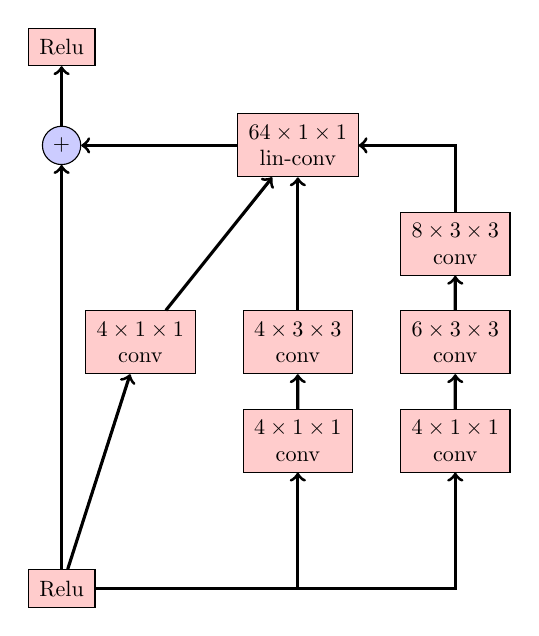
\begin{tikzpicture}[x=2cm, y=1.25cm]
		\tikzset{
			every node/.style={
				draw,
				scale=0.8,
				align=center,
				fill=black!20,
				inner sep=0.5em
			},
			conv/.style={
				rectangle,
				fill=red!20
			},
			nonlin/.style={
				rectangle,
				fill=red!20
			},
			plus/.style={
				circle,
				fill=blue!20,
				inner sep=0.25em
			},
			line/.style={
				->,
				line width=0.4mm
			}
		}

		\node[nonlin] (in) at (0.5, 0.5)
			{Relu};
		\node[nonlin] (out) at (0.5, 6)
			{Relu};
		\node[plus] (join) at (0.5, 5)
			{+};

		\node[conv] at (1, 3) (conv1)
			{$4 \times1  \times 1$\\ conv};

		\node[conv] at (2, 2) (conv2-1)
			{$4 \times 1 \times 1$\\ conv};
		\node[conv] at (2, 3) (conv2-2)
			{$4 \times 3 \times 3$\\ conv};

		\node[conv] at (3, 2) (conv3-1)
			{$4 \times 1 \times 1$\\ conv};
		\node[conv] at (3, 3) (conv3-2)
			{$6 \times 3 \times 3$\\ conv};
		\node[conv] at (3, 4) (conv3-3)
			{$8 \times 3 \times 3$\\ conv};

		\node[conv] at (2, 5) (conv4)
			{$64 \times 1 \times 1$\\ lin-conv};

		\draw[line] (in) -- (join);

		\draw[line] (in) -- (conv1);
		\draw[line] (in) -| (conv2-1);
		\draw[line] (in) -| (conv3-1);

		\draw[line] (conv2-1) -- (conv2-2);
		\draw[line] (conv3-1) -- (conv3-2);
		\draw[line] (conv3-2) -- (conv3-3);

		\draw[line] (conv1) -- (conv4);
		\draw[line] (conv2-2) -- (conv4);
		\draw[line] (conv3-3) |- (conv4);

		\draw[line] (conv4) -- (join);
		\draw[line] (join) -- (out);

	\end{tikzpicture}
	}
	\subfigure[Resnet B]
	{
	\begin{tikzpicture}[y=1.25cm]

		\node[nonlin] (in) at (0.5, 0.5)
			{Relu};
		\node[nonlin] (out) at (0.5, 6)
			{Relu};
		\node[plus] (join) at (0.5, 5)
			{+};

		\node[conv] at (1.5, 3) (conv1)
			{$192 \times 1 \times 1$\\ conv};

		\node[conv] at (2.5, 2) (conv2-1)
			{$128 \times 1 \times 1$\\ conv};
		\node[conv] at (2.5, 3) (conv2-2)
			{$160 \times 1 \times 7$\\ conv};
		\node[conv] at (2.5, 4) (conv2-3)
			{$192 \times 7 \times 1$\\ conv};

		\node[conv] at (1.5, 5) (conv4)
			{$1154 \times 1 \times 1$\\ conv};

		\draw[line] (in) -- (join);

		\draw[line] (in) -- (conv1);
		\draw[line] (in) -| (conv2-1);

		\draw[line] (conv2-1) -- (conv2-2);
		\draw[line] (conv2-2) -- (conv2-3);

		\draw[line] (conv1) -- (conv4);
		\draw[line] (conv2-3) |- (conv4);

		\draw[line] (conv4) -- (join);
		\draw[line] (join) -- (out);

	\end{tikzpicture}
	}
	\label{fig:res-ab}
	\caption{Modified Inception v4 resnets A/C}
\end{figure}

\begin{figure}[H]
	\centering
		\begin{tikzpicture}[y=1.25cm]

		\node[nonlin] (in) at (0.5, 0.5)
			{Relu};
		\node[nonlin] (out) at (0.5, 6)
			{Relu};
		\node[plus] (join) at (0.5, 5)
			{+};

		\node[conv] at (1.5, 3) (conv1)
			{$192 \times 1 \times 1$\\ conv};

		\node[conv] at (2.5, 2) (conv2-1)
			{$192 \times 1 \times 1$\\ conv};
		\node[conv] at (2.5, 3) (conv2-2)
			{$224 \times 3 \times 3$\\ conv};
		\node[conv] at (2.5, 4) (conv2-3)
			{$256 \times 3 \times 3$\\ conv};

		\node[conv] at (1.5, 5) (conv4)
			{$2048 \times 1 \times 1$\\ conv};

		\draw[line] (in) -- (join);

		\draw[line] (in) -- (conv1);
		\draw[line] (in) -| (conv2-1);

		\draw[line] (conv2-1) -- (conv2-2);
		\draw[line] (conv2-2) -- (conv2-3);

		\draw[line] (conv1) -- (conv4);
		\draw[line] (conv2-3) |- (conv4);

		\draw[line] (conv4) -- (join);
		\draw[line] (join) -- (out);

	\end{tikzpicture}
	\caption{Modified Inception v4 resnet C}
	\label{fig:res-c}
\end{figure}

\begin{figure}[H]
	\centering
	\subfigure[Reduction A]
	{
	\begin{tikzpicture}

		\node[nonlin] (in) at (0, 0)
			{Filter Concat};
		\node[nonlin] (out) at (0, 4)
			{Filter Concat};

		\node[conv] at (-1, 2) (conv1)
			{$32 \times 1 \times 1$\\ conv};

		\node[conv] at (0, 2) (conv2)
			{$32 \times 1 \times 1$\\ conv};

		\node[conv] at (1, 1) (conv3-1)
			{$48 \times 3 \times 3$\\ conv};
		\node[conv] at (1, 2) (conv3-2)
			{$48 \times 3 \times 3$\\ conv};
		\node[conv] at (1, 3) (conv3-3)
			{$48 \times 3 \times 3$\\ conv};

		\draw[line] (in) -| (conv1);
		\draw[line] (in) -- (conv2);
		\draw[line] (in) -- (conv3-1);

		\draw[line] (conv3-1) -- (conv3-2);
		\draw[line] (conv3-2) -- (conv3-3);

		\draw[line] (conv1) -- (out);
		\draw[line] (conv2) -- (out);
		\draw[line] (conv3-3) -- (out);
	\end{tikzpicture}
	}
	\subfigure[Reducation B]
	{
	\begin{tikzpicture}

		\node[nonlin] (in) at (0, 0)
			{Filter Concat};
		\node[nonlin] (out) at (0, 4)
			{Filter Concat};

		\node[conv] at (-1.5, 2) (conv1)
			{$32 \times 1 \times 1$\\ conv};

		\node[conv] at (-0.5, 1) (conv2-1)
			{$32 \times 1 \times 1$\\ conv};
		\node[conv] at (-0.5, 2) (conv2-2)
			{$32 \times 1 \times 1$\\ conv};

		\node[conv] at (0.5, 1) (conv3-1)
			{$32 \times 1 \times 1$\\ conv};
		\node[conv] at (0.5, 2) (conv3-2)
			{$32 \times 1 \times 1$\\ conv};

		\node[conv] at (1.5, 1) (conv4-1)
			{$48 \times 3 \times 3$\\ conv};
		\node[conv] at (1.5, 2) (conv4-2)
			{$48 \times 3 \times 3$\\ conv};
		\node[conv] at (1.5, 3) (conv4-3)
			{$48 \times 3 \times 3$\\ conv};

		\draw[line] (in) -| (conv1);
		\draw[line] (in) -- (conv2-1);
		\draw[line] (in) -- (conv3-1);
		\draw[line] (in) -| (conv4-1);

		\draw[line] (conv2-1) -- (conv2-2);
		\draw[line] (conv3-1) -- (conv3-2);

		\draw[line] (conv4-1) -- (conv4-2);
		\draw[line] (conv4-2) -- (conv4-3);

		\draw[line] (conv1) -- (out);
		\draw[line] (conv2-2) -- (out);
		\draw[line] (conv3-2) -- (out);
		\draw[line] (conv4-3) -- (out);

	\end{tikzpicture}
	}
	\label{fig:red}
	\caption{Modified Inception v4 reductions}
\end{figure}
\end{comment}

\end{solution}
% =========================================================
\HomeworkHeader{6 (Design)}{8}% homework number, problem number
% ---------------------------------------------------------
\begin{solution}
	Attempted. Inception v4 ended up being particularly difficult to implement.
	This revealed the importance of building small but robust blocks from which
	the entire network will eventually be composed. It also revealed the
	potential difficulty of debugging design errors, as Tensorflow exceptions
	were quite lengthy.
	\newline

	Ran into an issue where Tensorflow would raise \textsc{CUDA ERROR UNKNOWN}
	when trying to run on local GPU. Only solution was to reboot.
	Finally, I experimented with implementing GPU memory restrictions to
	improve training speed. My system uses two GTX970s which suffer a memory
	issue where $0.5$ of the total $4$GB runs significantly slower.
	Resticting memory usage and training on the secondary GPU that was not
	rendering X11 seemed to improve performance.
\end{solution}
% =========================================================
\HomeworkHeader{6 (Design)}{9}% homework number, problem number
% ---------------------------------------------------------
\begin{solution}
	I resorted to trying variations of and ResNext after Inception proved
	impractical to implement, however I was not able to exceed the accuracy of
	Resnet for CIFAR-10.
\end{solution}

\end{document}
